\documentclass[12pt]{article}
\usepackage{fancyhdr}
\usepackage{datetime}
\usepackage{enumitem}
\usepackage{float}
\usepackage{graphicx}
\graphicspath{ {images/} }
%\usepackage{showframe}

%custom variables
\newdate{date}{21}{10}{2016}
\newcommand{\hwNum}{3}
\newcommand{\assign}{Lab }
\newcommand{\class}{EC441: }
\newcommand{\name}{Daniel Andronov}


%header
\pagestyle{fancy}
\lhead{\name{}}
\chead{\thepage}
\rhead{\class{}\assign{}\hwNum{}}
\cfoot{\thepage}

\fancyheadoffset[LO,RE]{1pt}
\fancyheadoffset[RO,LE]{1pt}


%titlepage
\title{\class{}\assign{}\hwNum{}}
\author{\name{}}
\date{\displaydate{date}}


%addition settings
\topmargin=-0.45in
\evensidemargin=0in
\oddsidemargin=0in
\textwidth=6.5in
\textheight=9.0in
\headsep=0.25in


%offset the sections by 4
\setcounter{section}{4}
\setcounter{subsection}{2}

%adjusting vertical whitespace for the images at the top
\makeatletter
\setlength{\@fptop}{0pt}
\makeatother


%start the document
\begin{document}
\maketitle
\newpage

%webserver
\subsection{Web Server Program}

	\begin{figure}[h]
		\caption{The HTTP GET message forthe nonexistent \texttt{hhello\_world.html} file}
		\centering
		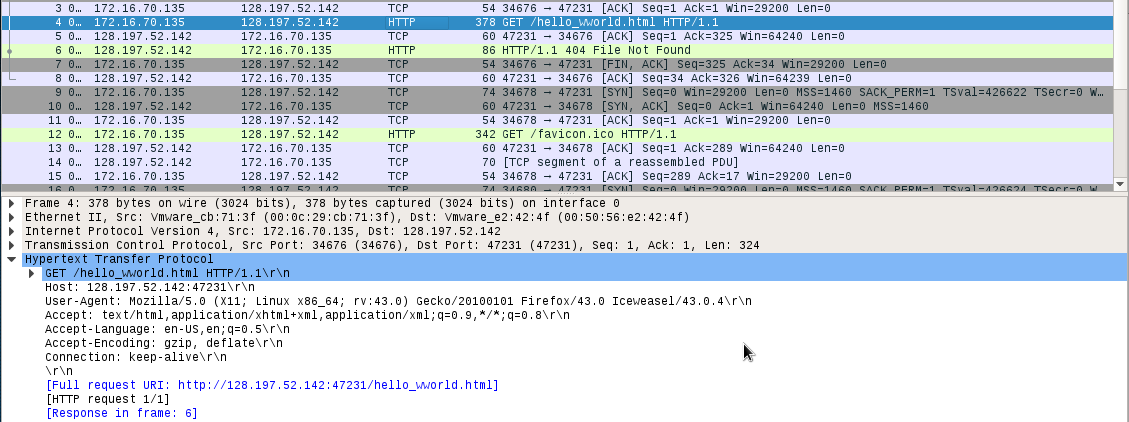
\includegraphics[width=\textwidth,height=\textheight,keepaspectratio,scale=0.5=0.5]{get_wrong}
	\end{figure}

	\begin{figure}[h]
		\caption{The HTTP GET response \texttt{404} message forthe nonexistent \texttt{hhello\_world.html} file}
		\centering
		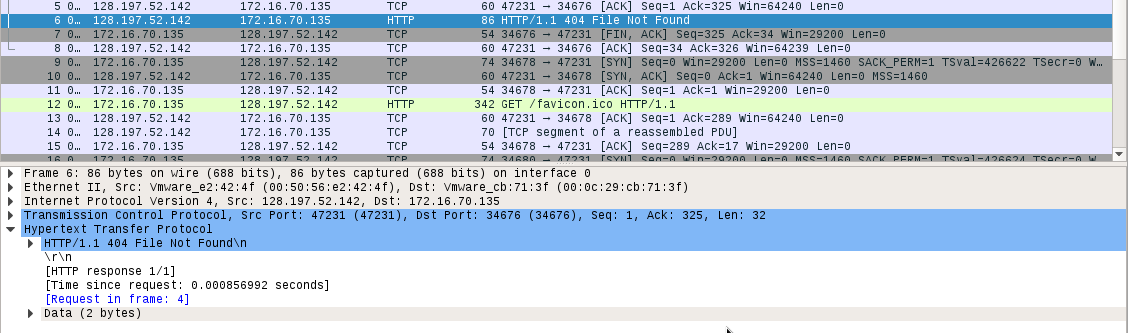
\includegraphics[width=\textwidth,height=\textheight,keepaspectratio,scale=0.5=0.5]{404_resp}
	\end{figure}

	\begin{figure}[h]
		\caption{The HTTP GET message forthe \texttt{hello\_world.html} file}
		\centering
		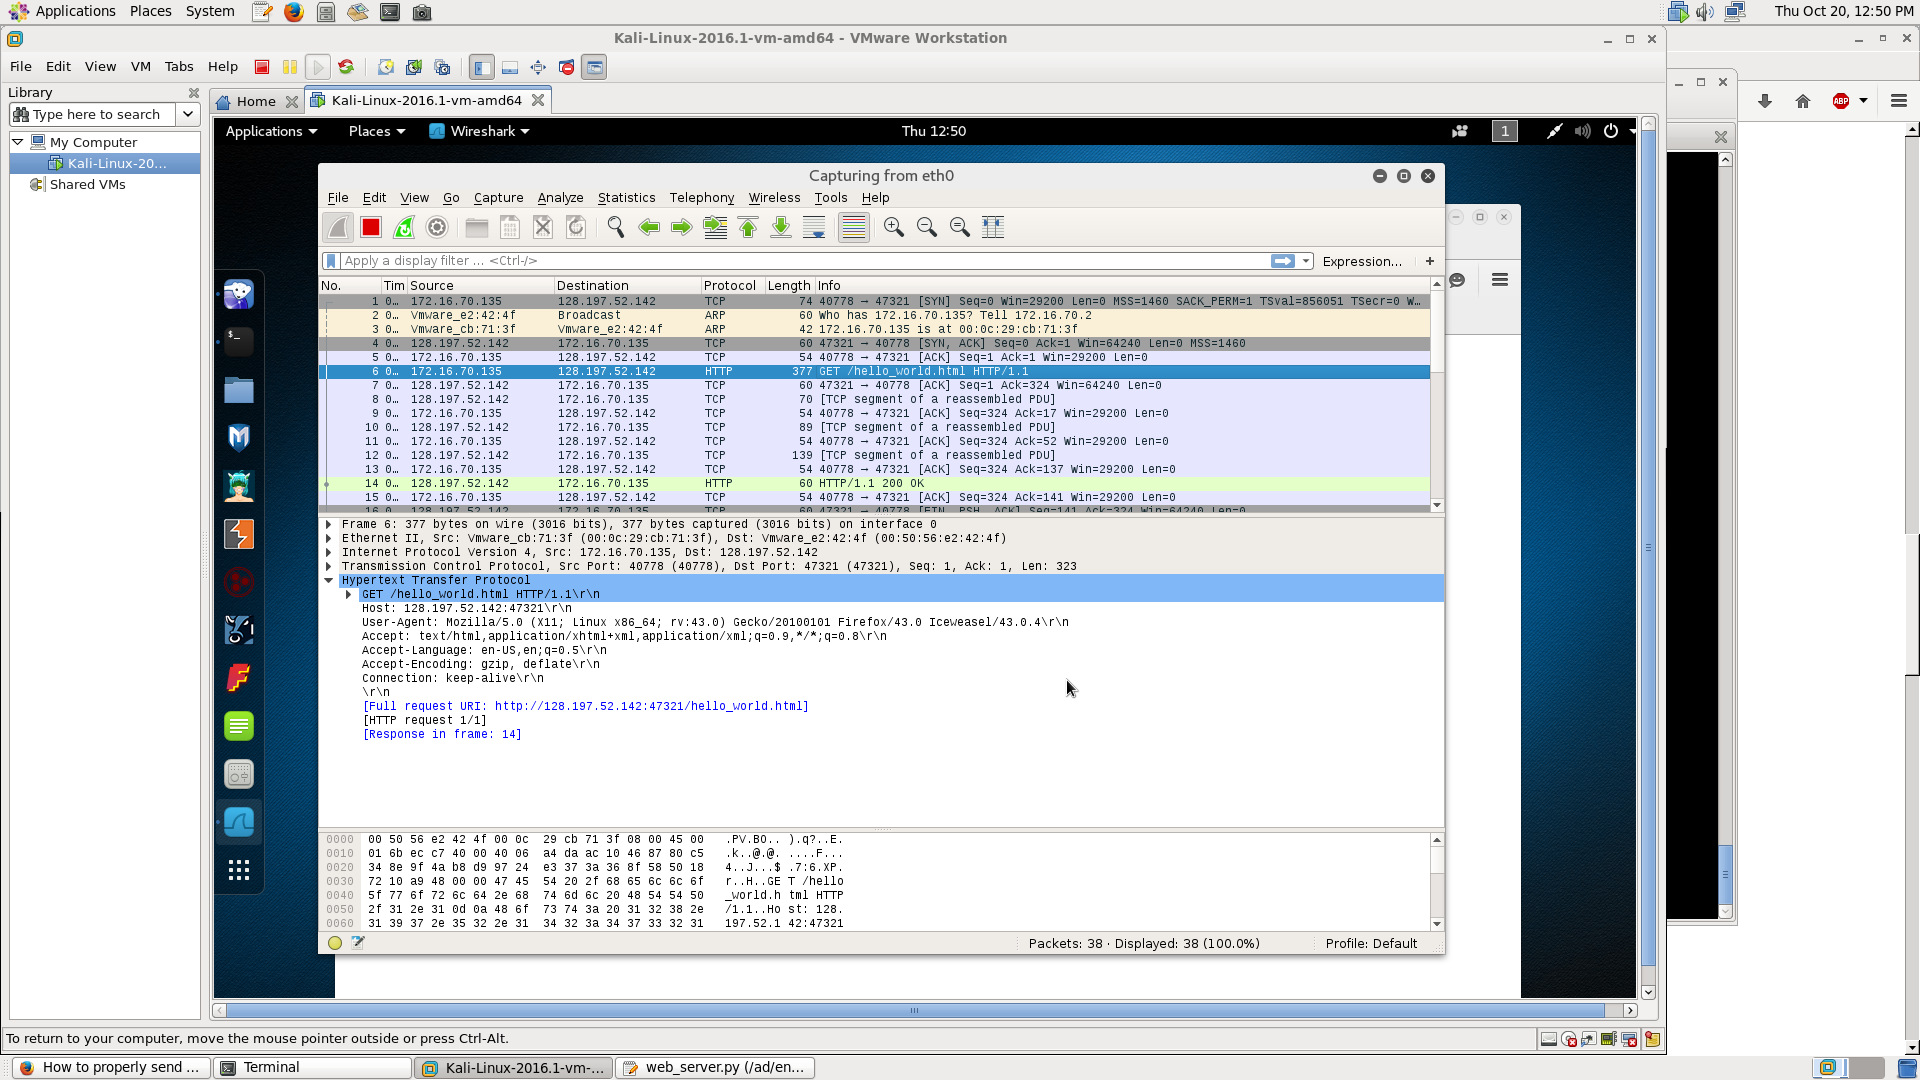
\includegraphics[width=\textwidth,height=\textheight,keepaspectratio,scale=0.5=0.5]{get_right}
	\end{figure}

	\begin{figure}[h]
		\caption{The HTTP GET response message forthe \texttt{hello\_world.html} file}
		\centering
		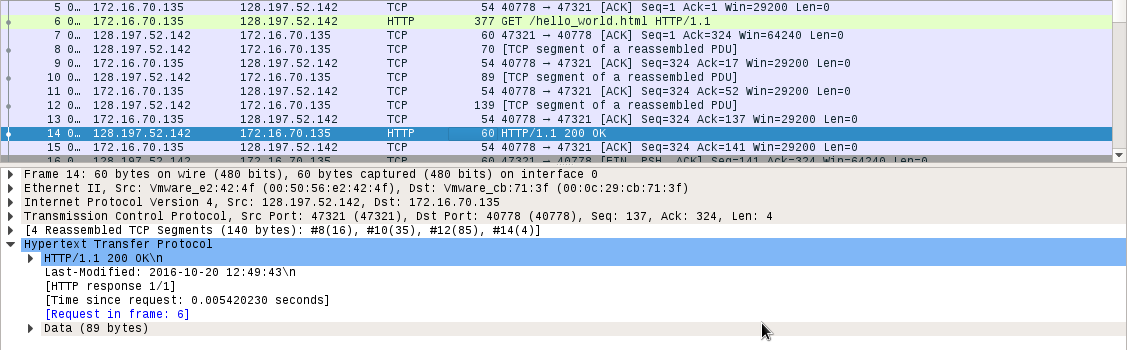
\includegraphics[width=\textwidth,height=\textheight,keepaspectratio,scale=0.5=0.5]{200_resp}
	\end{figure}
\clearpage
%favicon web_server
\subsection{Favicon Webserver}

	\begin{figure}[h]
		\caption{The HTTP GET message forthe \texttt{favicon.ioc} file}
		\centering
		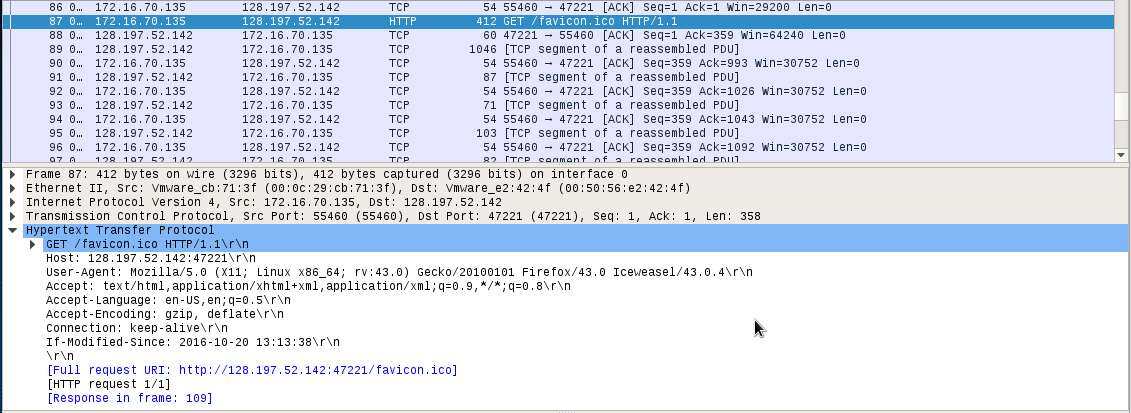
\includegraphics[width=\textwidth,height=\textheight,keepaspectratio,scale=0.5=0.5]{get_fav}
	\end{figure}

	\begin{figure}[h]
		\caption{The HTTP GET response message forthe \texttt{favicon.ico} file}
		\centering
		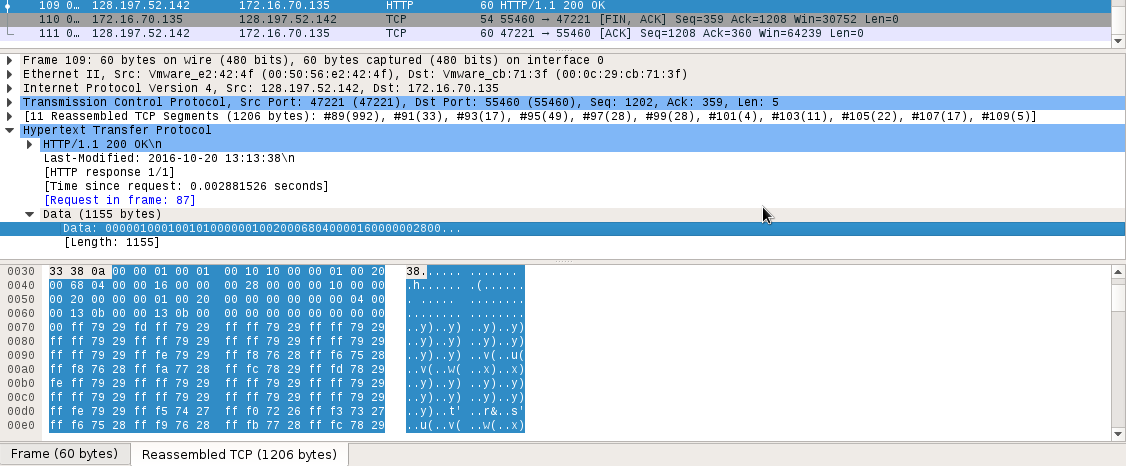
\includegraphics[width=\textwidth,height=\textheight,keepaspectratio,scale=0.5=0.5]{fav_resp}
	\end{figure}
\clearpage
%mail client
\subsection{Mail Client Program}

	\begin{figure}[h]
		\caption{The email sent to \texttt{andronov@bu.edu} via the mail client}
		\centering
		
\includegraphics[width=\textwidth,height=\textheight,keepaspectratio,scale=0.5=0.5]{self_mail}
	\end{figure}

	\begin{figure}[h]
		\caption{The commandline output when an unknown address is used}
		\centering
		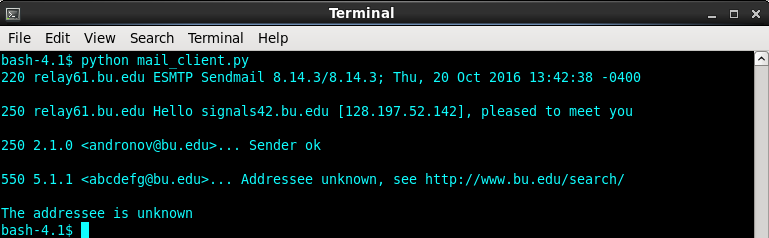
\includegraphics[width=\textwidth,height=\textheight,keepaspectratio,scale=0.5=0.5]{addr_unknown}
	\end{figure}

\end{document}
This is never printed